\chapter{Introduction}
\label{chapt:intro}
\chapterPage{
Model-driven engineering methodology and dynamically adaptive systems approach are combined to tackle challenges brought by systems nowadays.
After introducing these two software engineering techniques, we describe five problems that we identified for such systems: data uncertainty, actions with long-term effects, emergent behaviours of such systems, different evolution paces of the subparts, and the temporal dimension in their structures and behaviours.
We present the challenges that come with these problems.
Before describing the two contributions of this thesis, we scope to the addressed sub-challenges tackled.
}


\section{Context}
Utilities are introducing more and more \gls{ict} in the grid in order to face the new challenges of electricity supply~\cite{farhangi2010path, ipakchi2009grid, DBLP:journals/comsur/FangMXY12}.
These nowadays power grids are referred to as \gls{sg}.

In this document, we focus on the \textbf{\gls{shealing}} capacity of such grids.
A \gls{shealingSyst} can automatically repair any incident, software or hardware, at runtime~\cite{DBLP:journals/computer/KephartC03}.
For example, a smart grid can optimize the power flow to deal with failures of transformers\footnote{Transformers change the voltage in cables.}~\cite{DBLP:journals/comsur/FangMXY12}.
In this way, the incident will impact as few users as possibles, ideally none. 

This healing mechanism can be performed only if the smart grid has a deep understanding of itself and its environment.
To tame their complexity, a common approach in software engineers is to use an \textbf{abstraction} mechanism.
Abstractions provide an illuminating description of systems, their behaviours, or their environment.
For example, Hartmann~\etal \cite{DBLP:conf/smartgridcomm/0001FKTPTR14} provide a class diagram that describes the smart grid topology, when it uses power-line communications\footnote{Data are sent through cables that also distribute electricity.}.

\bigskip

More generally, a \gls{shealing} is a \textbf{\gls{sadapt}}. 
Cheng \etal define \glspl{sadapt} as \textquote{systems that are able to adjust their behaviour in response to their perception of the environment and the system itself}~\cite{DBLP:conf/dagstuhl/ChengLGIMABBBCSDFGGGKKKLMMMPSTTWW09}.
Jeffrey O. Kephart and David M. Chess~\cite{DBLP:journals/computer/KephartC03} laid the groundwork of this approach, based on an IBM white paper~\cite{computing2006architectural}.
Since then, it has been used in different domain~\cite{DBLP:journals/corr/abs-1904-01518} such as cloud infrastructure~\cite{DBLP:conf/icac/JavadiG17, OpenStack:Watcher:Wiki, DBLP:conf/icse/BarnaKFL17} or \gls{cps}~\cite{DBLP:conf/icac/LalandaGC17, DBLP:conf/cbse/FouquetMFBPJ12, DBLP:conf/smartgridsec/0001FKNT14}.

\textbf{\Gls{mde}} uses the abstraction mechanism to facilitate the development of nowadays software~\cite{DBLP:journals/computer/Schmidt06, DBLP:conf/ifm/Kent02, DBLP:series/synthesis/2017Brambilla}.
This methodology can be applied to different stages of software development.
In this thesis, we focus on one of its paradigm: \textbf{\gls{m@rt}}~\cite{DBLP:journals/computer/BlairBF09, DBLP:journals/computer/MorinBJFS09}.
The state of the system or its environment, as well as its behaviour, are reflected in a model, used for analysis.
Developers can use this paradigm to implement \glspl{adptSyst}~\cite{DBLP:journals/computer/MorinBJFS09, DBLP:conf/smartgridsec/0001FKNT14}.

\bigskip

Whereas smart grids introduce more and more automation capacity, human interventions are still required.
First, information gathered by smart grids is therefore not always known with absolute confidence.
Second, smart grids reconfigurations are not immediate, and their effects are not instantaneously measured.
Third, smart grids behaviour is emergent~\cite{zio2011uncertainties}, \ie it cannot be entirely known at design time.

Most fuses are manually open and close by technicians rather than automatically modified.
Then, technicians manually report the modifications done on the grid.
Due to human mistakes, this results in errors.
The grid topology is thus uncertain.
This uncertainty is propagated to the load approximation, used to detect overloads in the grid.
Wrong reconfigurations might be triggered, which could be even worse than if no change would have been applied.

Reconfiguring a smart grid implied to change the power flow.
It is done by connecting or disconnecting specific cables.
That is, opening or closing fuses.
As said before, a technician needs to drive physically to the fuse location to modify its state.
Besides, in the case of the Luxembourg smart grid, meters send energy measurement every 15 mins, non-synchronously.
Between the time a reconfiguration of the smart grid is decided, and the time the effects are measured, a delay of at least 15 mins occurs.
On the other hand, an incident should be detected in the next minutes.
If the adaptation process does not consider this difference of paces, it can cause repeated decisions.

Smart grid behaviour is affected by several factors that cannot be controlled by the grid manager.
One example is the weather condition.
Smart grids rely on an energy production that is distributed over several actors.
For instance, users, who were mainly consumers before, now produce energy by adding solar panels on the roof of their houses.
The production of such energy depends on the weather, and even on the season\footnote{The angle of the sun has an impact on the amount of energy produced by solar panels. This angle varies according to the season.}.
Another example is the increasing adoption of electric vehicles, which de facto drastically increase the consumption of electricity during the night.
Ignoring this characteristic of \gls{adptSyst} may result in suboptimal situations that can be understood with difficulties.
\section{Défis}

%During our study, we have identified five characteristics of \glspl{adptSyst} that bring challenges to the software engineering research community.
%First, information gathered is not always known with absolute confidence.
%Second, reconfigurations may not be immediate, and their effects are not instantaneously measured.
%Third, system behaviour may be emergent~\cite{zio2011uncertainties}, \ie it cannot be entirely known at design time.
%Four, the different sub-parts of the system do not evolve at the same rate.
%Five, structure and behaviour of systems have a time dimension.
%The last one has been published in our vision paper regarding time awareness in \gls{mde}~\cite{DBLP:conf/models/Benelallam0MFBB17}.
%We detailed them in this section.
%
Au cours de notre étude, nous avons identifié cinq caractéristiques des systèmes adaptatifs qui posent des défis pour la recherche en génie logiciel. 
Premièrement, l'information recueillie n'est pas toujours connue avec une confiance absolue. 
Deuxièmement, les reconfigurations peuvent ne pas être immédiates et leurs effets ne sont pas instantanément mesurés. 
Troisièmement, le comportement du système peut être émergent~\cite{zio2011uncertainties}, c'est-à-dire qu'il ne peut être entièrement connu au moment de la conception. 
Quatrièmement, les différentes sous-parties du système n'évoluent pas au même rythme. 
Cinquièmement, la structure et le comportement des systèmes ont une dimension temporelle. 
La dernière a été publiée dans notre document de vision concernant la prise de conscience du temps dans l'IDM~\cite{DBLP:conf/models/Benelallam0MFBB17}. 
Nous les avons détaillés dans cette section.

\subsection{Ingénierie de logiciels sensibles à l'incertitude}
\label{sec_french_challenges_duc}

\begin{figure}
	\centering
	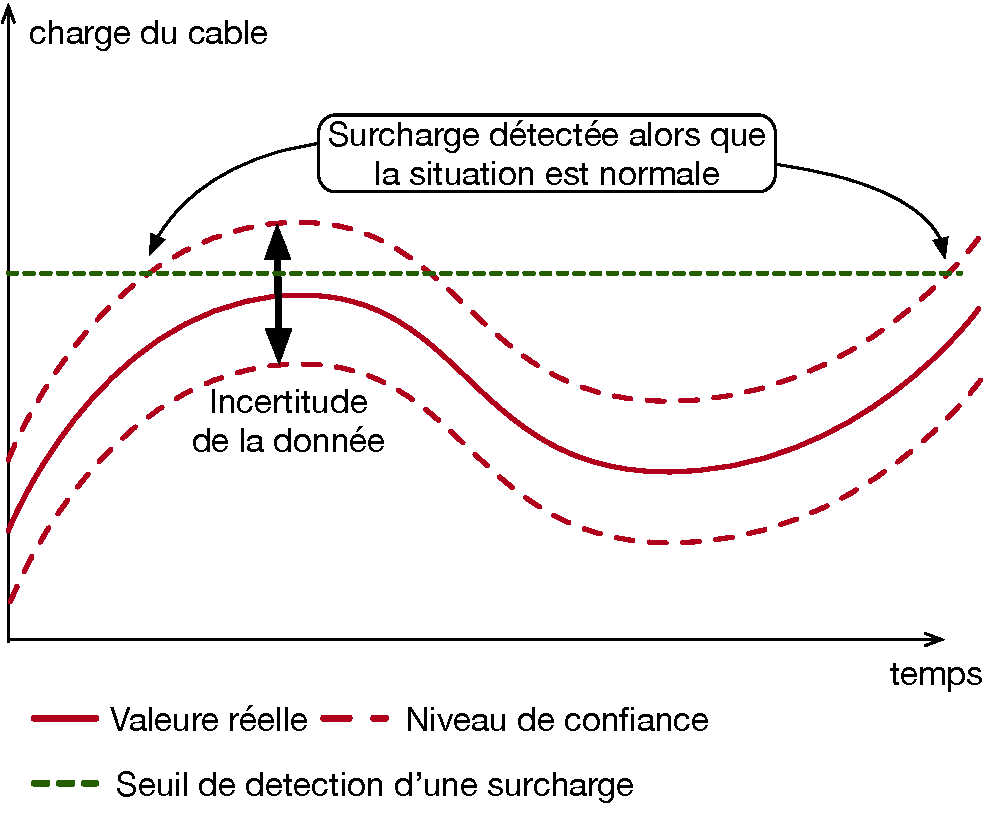
\includegraphics[width=.6\linewidth]{img/apdx-french/challenges/duc}
	\caption{Illustration du problème causé par l'incertitude des données}
	\label{fig_french_chal_duc}
\end{figure}

%Most fuses are manually opened and closed by technicians rather than automatically modified.
%Then, technicians manually report the modifications done on the grid.
%Due to human mistakes, this results in errors.
%The grid topology is thus uncertain.
%This uncertainty is propagated to the load approximation, used to detect overloads in the grid.
%Wrong reconfigurations might be triggered, which could be even worse than if no change would have been applied.
%
La plupart des fusibles sont ouverts et fermés manuellement par les techniciens plutôt que modifiés automatiquement. 
Ensuite, les techniciens rapportent manuellement les modifications effectuées sur la grille.
En raison d'erreurs humaines, il en résulte des erreurs.
La topologie de la grille est donc incertaine.
Cette incertitude se propage à l'approximation de la charge, utilisée pour détecter les surcharges dans le réseau.
De mauvaises reconfigurations pourraient être déclenchées, ce qui pourrait être encore pire que si aucun changement n'avait été appliqué.

%More generally, \textbf{data are, almost by definition, uncertain and developers work with estimates in most cases}~\cite{DBLP:conf/asplos/BornholtMM14, metrology2008evaluation, DBLP:journals/tkde/AggarwalY09}.
%The uncertainty may be explained by how data are collected.
%We can distinguish three categories: sensors, humans, and results of computations.
%Sensors (software or hardware) always estimate the value and have a precision value due to the method of measurement~\cite{metrology2008evaluation, DBLP:conf/asplos/BornholtMM14}.
%Humans are error-prone.
%Computations can either give an approximation or be based on uncertain data.
%This uncertainty is then propagated through all steps until the final result.
%
Plus généralement, les données sont, presque par définition, incertaines et les développeurs travaillent avec des estimations dans la plupart des cas~\cite{DBLP:conf/asplos/BornholtMM14, metrology2008evaluation, DBLP:journals/tkde/AggarwalY09}.
L'incertitude peut s'expliquer par la façon dont les données sont recueillies.
On peut distinguer trois catégories : les capteurs, les humains et les résultats des calculs.
Les capteurs (logiciels ou matériels) estiment toujours la valeur et ont une valeur de précision grâce à la méthode de mesure~\cite{metrology2008evaluation, DBLP:conf/asplos/BornholtMM14}.
Les humains sont sujets à l'erreur.
Les calculs peuvent soit donner une approximation, soit être basés sur des données incertaines.
Cette incertitude se propage ensuite à travers toutes les étapes jusqu'au résultat final.

%For a specific domain, this uncertainty may impact the understanding of the real situation as depicted in~\Cref{fig:intro:chal:duc}.
%For example, the uncertainty of the \gls{cpu} clock is too low to damage the percentage load of the processor.
%However, the uncertainty of the cable load in a smart grid may trigger false detection of an overload, as depicted in~\Cref{fig:intro:chal:duc}.
%\textbf{If the data uncertainty can mislead the understanding of a system behaviour or state, then developers should implement an uncertainty-aware system.}
%For \glspl{adptSyst}, this lack of confidence may trigger suboptimal adaptations.
%
Pour un domaine spécifique, cette incertitude peut avoir une incidence sur la compréhension de la situation réelle, comme le montre la~\cref{fig_french_chal_duc}. 
Par exemple, l'incertitude de l'horloge CPU est trop faible pour endommager le pourcentage de charge du processeur. 
Cependant, l'incertitude de la charge du câble dans un réseau intelligent peut déclencher une fausse détection d'une surcharge, comme le montre la~\cref{fig_french_chal_duc}. 
Si l'incertitude des données peut induire en erreur la compréhension du comportement ou de l'état d'un système, les développeurs doivent mettre en œuvre un système conscient de l'incertitude. 
Pour les systèmes adaptatifs, ce manque de confiance peut entraîner des adaptations sous-optimales.

%Therefore, we argue that \gls{duc} impacts all the development stages of software, from the design to the execution.
%Among the different stages, in this thesis we focus on the design one.
%We firmly think that design techniques should provide mechanisms to help developers abstract and manipulating uncertain data.
%
Par conséquent, nous soutenons que l'incertitude des données a une incidence sur toutes les étapes du développement d'un logiciel, de la conception à l'exécution.
Parmi les différentes étapes de cette thèse, nous nous concentrons sur celle de la conception.
Nous croyons fermement que les techniques de conception devraient fournir des mécanismes pour aider les développeurs à abstraire et à manipuler des données incertaines.

%The literature provides approaches to help engineers reason or manipulate \gls{duc}, or at least probability distributions.
%For example, believe func-\linebreak{}tions~\cite{shafer1992dempster} help to reduce this uncertainty by combining several sources of data.
%The probabilistic programming~\cite{DBLP:conf/icse/GordonHNR14} community provide frameworks and languages~\cite{url:InferNET18, baudin2017openturns} to propagate probabilities through computations.
%
La littérature fournit des approches pour aider les ingénieurs à raisonner ou à manipuler les données sans certitude, ou du moins les distributions de probabilité.
Par exemple, les fonctions de croyances~\cite{shafer1992dempster} aident à réduire cette incertitude en combinant plusieurs sources de données.
La communauté de programmation probabilistic~\cite{DBLP:conf/icse/GordonHNR14} fournit des \textit{frameworks} et des langages de programmation~\cite{url:InferNET18, baudin2017openturns} pour propager les probabilités lors des calculs.

%However, from the best of our knowledge, no study has been done to evaluate the impact of data uncertainty on the development of software.
%The following challenge still remains an open question for the software engineering community:
%\vspace{-2em}
%\highlightbox{How to engineer uncertainty-aware software (design, implement, test, and validate)?}
%
Cependant, à notre connaissance, aucune étude n'a été effectuée pour évaluer l'impact de l'incertitude des données sur le développement des logiciels. 
Le défi suivant demeure une question ouverte pour la communauté du génie logiciel :
\vspace{-2em}
\highlightbox{Comment concevoir des logiciels sensibles à l'incertitude (conception, mise en œuvre, test et validation) ?}

\subsection{Raisonnement sur les actions à long terme}
\label{sec_french_challenges_longTermAct}

\begin{figure}
	\centering
	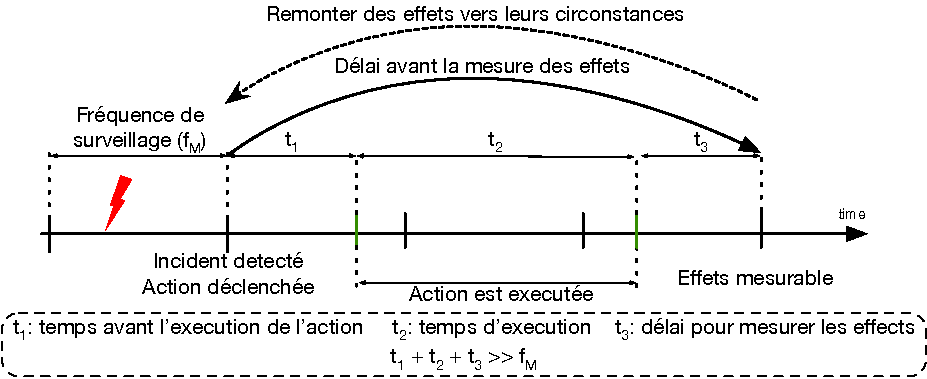
\includegraphics[width=0.9\linewidth]{img/apdx-french/challenges/longTermAct}
	\caption{Illustration d'une action à long terme}
	\label{fig_french_chal_longTermAct}
\end{figure}

%Reconfiguring a smart grid implies to change the power flow by opening or closing fuses.
%As said before, technicians need to drive physically to fuse locations to modify their states.
%In the case of the Luxembourg smart grid, meters send energy measurement every 15 min, non-synchronously.
%Therefore, between the time a reconfiguration of the smart grid is decided, and the time the effects are measured, a delay of at least 15 min occurs.
%On the other hand, an incident should be detected in the next minutes.
%If the adaptation process does not consider this difference of rates, it can cause repeated decisions.
%
La reconfiguration d'un réseau intelligent implique de modifier le flux de puissance en ouvrant ou en fermant les fusibles. 
Comme nous l'avons déjà dit, les techniciens doivent se rendre physiquement sur les lieux des fusibles pour modifier leur états. 
Dans le cas du réseau intelligent luxembourgeois, les compteurs envoient des mesures d'énergie toutes les 15 minutes, de manière non synchrone. 
Par conséquent, entre le moment où une reconfiguration du réseau intelligent est décidée et le moment où les effets sont mesurés, un retard d'au moins 15 minutes se produit. 
D'autre part, un incident devrait être détecté dans les minutes qui suivent. 
Si le processus d'adaptation ne tient pas compte de cette différence de rythme, il peut entraîner des décisions répétées.

%More generally, a difference may exist between the monitoring frequency of the time for action effects to be measured.
%One cause of this is what we call \glspl{longTermAct} in this document, illustrated in~\Cref{fig:intro:chal:longTermAct}.
%A \gls{longTermAct} is defined as an \gls{action} that takes time to be executed  (delay to be executed and execution time) or that have long-term effects.
%A second cause is an impossibility to reduce the monitoring frequency since systems must be reactive in some cases.
%This difference in rates may damage the decision process.
%
De façon plus générale, il peut exister une différence entre la fréquence de surveillance et le temps nécessaire pour mesurer les effets de l'action. 
L'une des causes de cette différence est ce que nous appelons les actions à long terme dans ce document, illustrées à la~\cref{fig_french_chal_longTermAct}. 
Une action à long terme est définie comme une action qui prend du temps à être exécutée (retard à exécuter et temps d'exécution) ou qui a des effets à long terme.
Une deuxième cause est l'impossibilité de réduire la fréquence de surveillance puisque les systèmes doivent être réactifs dans certains cas.
Cette différence de taux peut nuire au processus décisionnel.

%Therefore, we argue that \textbf{decision-making processes should consider this delay if the frequency of the monitoring stage is lower than the time of action effects to be measurable}.
%From the best of our knowledge, none of the approaches allows developers implementing such tools.
%One open challenge for the research community is thus:
%\vspace{-2em}
%\highlightbox{How to model, store, and query long-term actions with their effects?}
Par conséquent, nous soutenons que les processus décisionnels devraient tenir compte de ce délai si la fréquence de l'étape de surveillance est inférieure à la durée des effets de l'action pour pouvoir être mesurée. 
A notre connaissance, aucune des approches ne permet aux développeurs d'implémenter de tels outils. 
L'un des défis ouverts pour la communauté des chercheurs est donc le suivant :
\vspace{-2em}
\highlightbox{Comment modéliser, stocker et interroger les actions à long terme avec leurs effets ?}

\subsection{Diagnostic du processus d'adaptation}
\label{sec_french_challenges_diagnosis}

%\Gls{sg} \gls{behaviour} is affected by several factors that cannot be controlled by the grid manager.
%One example is weather conditions.
%\Glspl{sg} rely on an energy production distributed over several actors.
%For instance, users, who were mainly consumers before, can now produce energy by adding solar panels on the roof of their houses.
%The production of such energy depends on the weather, and even on the season\footnote{The angle of the sun has an impact on the amount of energy produced by solar panels. This angle varies according to the season.}.
%Despite this stochasticity of the \gls{behaviour}, engineers need to implement an adaptation process, that can lead to suboptimal grid configuration.
%
Le comportement du réseau intelligent est affecté par plusieurs facteurs qui ne peuvent pas être contrôlés par le gestionnaire de réseau. 
Les conditions météorologiques en sont un exemple. Les réseaux intelligents reposent sur une production d'énergie répartie entre plusieurs acteurs. 
Par exemple, les utilisateurs, qui étaient auparavant principalement des consommateurs, peuvent maintenant produire de l'énergie en ajoutant des panneaux solaires sur le toit de leur maison. 
La production de cette énergie dépend de la météo, et même de la saison\footnote{L'angle du soleil a un impact sur la quantité d'énergie produite par les panneaux solaires. Cet angle varie selon la saison.}. 
Malgré cette stochasticité du comportement, les ingénieurs doivent mettre en œuvre un processus d'adaptation qui peut conduire à une configuration de grille sous-optimale.

%Faced with growingly complex and large-scale software systems (e.g. smart grid systems), we can all agree that the presence of residual defects becomes unavoidable~~\cite{DBLP:conf/icse/BarbosaLMJ17, DBLP:conf/icse/MongielloPS15, DBLP:conf/icse/HassanBB15}. 
%Even with a meticulous verification or validation process, it is very likely to run into an unexpected behaviour that was not foreseen at design time. 
%Alone, existing formal modelling and verification approaches may not be sufficient to anticipate these failures~\cite{DBLP:conf/icse/TaharaOH17}. 
%As such, complementary techniques need to be proposed to locate the anomalous behaviour and its origin in order to handle it in a safe way.
%
Face à des systèmes logiciels de plus en plus complexes et à grande échelle (par exemple les systèmes de réseaux intelligents), nous pouvons tous convenir que la présence de défauts résiduels devient inévitable~\cite{DBLP:conf/icse/BarbosaLMJ17, DBLP:conf/icse/MongielloPS15, DBLP:conf/icse/HassanBB15}.
Même avec un processus méticuleux de vérification ou de validation, il est très probable de se heurter à un comportement inattendu qui n'était pas prévu au moment de la conception.
À elles seules, les approches formelles de modélisation et de vérification existantes peuvent ne pas être suffisantes pour anticiper ces défaillances~\cite{DBLP:conf/icse/TaharaOH17}.
A ce titre, des techniques complémentaires doivent être proposées pour localiser le comportement anormal et son origine afin de le manipuler en toute sécurité.

%Bencomo~\etal~\cite{DBLP:conf/iceccs/BencomoWSW12} argue that comprehensive explanation about the system behaviour contributes drastically to the quality of the diagnosis, and eases the task of troubleshooting the system behaviour. 
%To enable this, as shown in~\Cref{fig:intro:chal:longTermAct}, we believe that adaptive software systems should be equipped with traceability management facilities to link the decisions made to their \textbf{(i) circumstances, that is to say, the history of the system states and the targeted requirements, and (ii) the performed actions with their impact(s) on the system}.
%In particular, an \textbf{adaptive system should keep a trace of the relevant historical events}.
%Additionally, it should be able to \textbf{trace the goals intended to be achieved by the system to the adaptations and the decisions that have been made, and vice versa}. 
%Finally, in order to enable developers to interact with the system in a clear and understandable way, appropriate abstraction to \textbf{enable the navigation of the traces and their history should also be provided}.
%In other words, one global challenge that remains unaddressed is:
%\vspace{-2em}
%\highlightbox{How to trace back adaptation decision effects to their circumstances?}
Bencomo~\etal~\cite{DBLP:conf/iceccs/BencomoWSW12} soutiennent qu'une explication complète du comportement du système contribue de manière drastique à la qualité du diagnostic et facilite la tâche de dépannage du comportement du système. 
Pour ce faire, comme le montre la~\cref{fig_french_chal_longTermAct}, nous pensons que les systèmes logiciels adaptatifs devraient être dotés d'installations de gestion de la traçabilité pour relier les décisions prises à (i) leur  situation, c'est-à-dire l'historique des états du système et les exigences visées, et (ii) les actions réalisées et leur(s) impact(s) sur le système. 
En particulier, un système adaptatif devrait conserver une trace des événements historiques pertinents. 
En outre, il devrait être en mesure de lier les objectifs que le système entend atteindre aux adaptations et aux décisions qui ont été prises, et vice versa. 
Enfin, afin de permettre aux développeurs d'interagir avec le système d'une manière claire et compréhensible, une abstraction appropriée pour permettre la navigation des traces et leur historique devrait également être fournie. 
En d'autres termes, un défi qui n'a pas encore été relevé est le suivant :
\vspace{-2em}
\highlightbox{Comment faire remonter les effets des décisions d'adaptation à leur situation ?}

\subsection{Modélisation des états incohérents des systèmes}
%Every meter sends consumption and production data every 15 min.
%However, this collection is not synchronous.
%That is, not all meters send their data at the same timestamp.
%The global system, which receives all data, has not thus a global vision with the same freshness for all the part of the grid.
%Electricity data are volatile: a peak or a drop may happen in less than a minute due to, for instance, the starting or the finishing of a washing machine.
%Reconfiguration of the grid may thus be suboptimal due to outdated information.
%
Chaque compteur envoie des données de consommation et de production toutes les 15 minutes. 
Cependant, cette collection n'est pas synchrone. 
Autrement dit, tous les compteurs n'envoient pas leurs données au même moment. 
Le système global, qui reçoit toutes les données, n'a donc pas une vision globale avec la même fraîcheur pour toute la partie de la grille. 
Les données électriques sont volatiles : un pic ou une baisse peut survenir en moins d'une minute en raison, par exemple, du démarrage ou de la finition d'une machine à laver. 
La reconfiguration de la grille peut donc être sous-optimale en raison d'informations périmées.

%\textbf{Different parts of a system may evolve at different rates.}
%Some systems are heterogeneous in terms of hardware and software.
%This diversity results in different evolution or reaction rates.
%For example, if some components are working on batteries, they will have a sleep cycle to save energy.
%Contrary, if some others are running connected directly to a power source, they can react faster.
%
Les différentes parties d'un système peuvent évoluer à des rythmes différents. 
Certains systèmes sont hétérogènes en termes de matériel et de logiciels. 
Cette diversité se traduit par des évolutions ou des taux de réaction différents. 
Par exemple, si certains composants fonctionnent sur batteries, ils auront un cycle de sommeil pour économiser de l'énergie. 
A l'inverse, si d'autres sont connectés directement à une source d'énergie, ils peuvent réagir plus rapidement.

%Despite this difference of rates, a global vision of a system at a precise time point may be still required.
%The vision should deal with data that have different freshness.
%For example, the adaptation process may require a global view of the system.
%In the worst case, some data would be outdated and cannot be used.
%
Malgré cette différence de rythmes, une vision globale d'un système à un moment précis peut encore être nécessaire. 
La vision devrait porter sur des données qui ont une fraîcheur différente. 
Par exemple, le processus d'adaptation peut nécessiter une vision globale du système. 
Dans le pire des cas, certaines données seraient périmées et ne pourraient être utilisées.

%When designing the adaptation process, engineers need thus solutions to deal with an inconsistent system state.
%One solution can, for example, seamlessly estimate what should be the current value of outdated data.
%One global challenge for the software engineering community is therefore:
%\vspace{-2em}
%\highlightbox{How to represent, query, and store inconsistent system states and behaviours?}
Lors de la conception du processus d'adaptation, les ingénieurs ont donc besoin de solutions pour faire face à un état inconsistant du système. 
Une solution peut, par exemple, estimer de façon transparente ce que devrait être la valeur actuelle de données périmées. 
Un défi pour la communauté du génie logiciel est donc :
\vspace{-2em}
\highlightbox{Comment représenter, interroger et stocker des états et des comportements système incohérents ?}

\subsection{Modélisation des données temporelles et interconnectées}
%Power flow is impacted by consumption and production of users, and by the modifications of the topology.
%Knowing the last status of the grid is as important as knowing how it evolves.
%Based on the evolution, the grid operator can predict any future incidents, like overloads.
%It could also compare this evolution of behaviour with a normal one to detect, for example, any malicious behaviour.
%
Le flux d'énergie est influencé par la consommation et la production des utilisateurs, ainsi que par les modifications de la topologie. 
Connaître le dernier statut de la grille est aussi important que savoir comment elle évolue.
En fonction de l'évolution, l'exploitant du réseau peut prévoir tout incident futur, comme une surcharge.
Il pourrait également comparer cette évolution de comportement avec une évolution normale pour détecter, par exemple, tout comportement malveillant.

%\textbf{Evolution of systems is inherently linked with a time dimension.}
%Evolution and time are two related concepts.
%For some systems, not only the last states are important but also how they evolve.
%Then, analysis processes will investigate this evolution to know if it is a normal one or not.
%They can also use this evolution to predict how systems will evolve.
%Based on these predictions, they can proact on future incidents in the system.
%
L'évolution des systèmes est intrinsèquement liée à une dimension temporelle.
Evolution et temps sont deux concepts liés.
Pour certains systèmes, non seulement les derniers états sont importants, mais aussi leur évolution.
Ensuite, les processus d'analyse examineront cette évolution pour savoir si elle est normale ou non.
Ils peuvent aussi utiliser cette évolution pour prédire comment les systèmes vont évoluer.
En se basant sur ces prévisions, ils peuvent prévoir les incidents futurs dans le système.

%Decisions are not made upon the last state of the system but how it evolves.
%The analysis process should thus navigate both in the structure of the system and its behaviour over time.
%\textbf{Engineers need efficient tooling to structure, represent, query, and store temporal and interconnected data on a large scale.}
%
Les décisions ne sont pas prises en fonction du dernier état du système, mais en fonction de son évolution.
Le processus d'analyse doit donc naviguer à la fois dans la structure du système et dans son comportement dans le temps.
Les ingénieurs ont besoin d'outils efficaces pour structurer, représenter, interroger et stocker des données temporelles et interconnectées à grande échelle.

%Time in software engineering is not a new challenge.
%For example, Riviera \etal \cite{DBLP:conf/models/RiveraRV08} have already identified time as a challenge for the \gls{mde} community.
%Different approaches have been defined~\cite{DBLP:conf/sle/BousseCCGB15, DBLP:conf/sle/KansoT12, DBLP:conf/icse/KoegelH10, DBLP:conf/seke/0001FNMKT14}.
Le temps n'est pas un nouveau défi pour le génie logiciel . 
Par exemple, Riviera~\etal \cite{DBLP:conf/models/RiveraRV08} ont déjà identifié le temps comme un défi pour la communauté de l'IDM. 
Différentes approches ont été définies~\cite{DBLP:conf/sle/BousseCCGB15, DBLP:conf/sle/KansoT12, DBLP:conf/icse/KoegelH10, DBLP:conf/seke/0001FNMKT14}.

%However, we notice that research efforts made by the \gls{mde} community did not focus on the modelling, persistence, and processing of evolving data.
%Thomas Hartmann started addressing these challenging in his PhD thesis~\cite{DBLP:phd/basesearch/Hartmann16}.
%The final global challenge, not fully addressed, is thus:
%\vspace{-2em}
%\highlightbox{How to structure, represent, query, and store efficiently temporal data on a large scale?}
Cependant, nous remarquons que les efforts de recherche déployés par la communauté des EMM n'étaient pas axés sur la modélisation, la persistance et le traitement des données en évolution. 
Thomas Hartmann a commencé à aborder ces défis dans sa thèse de doctorat~\cite{DBLP:phd/basesearch/Hartmann16}. 
Le dernier défi, qui n'est pas entièrement relevé, est donc :
\vspace{-2em}
\highlightbox{Comment structurer, représenter, requêter et stocker efficacement des données temporelles à grande échelle ?}
\section{Scope of the thesis}
\label{sec:intro:scope}

Among all the challenges described in the previous section, this thesis focuses on three of them: \gls{duc} (\Cref{sec:intro:challenges:duc}), \glspl{longTermAct} (\Cref{sec:intro:challenges:longTermAct}), and error-prone adaptation process (\Cref{sec:intro:challenges:diagnosis}).
More precisely, we address three sub-problems of these challenges.

Managing uncertainty requires significant expertise in probability and statistics theory.
The literature provides different solutions to manage uncertainty~\cite{zadeh1996fuzzy,metrology2008evaluation,shafer1992dempster}.
The application of these techniques requires a deep understanding of the underlying theories and is a time-consuming task~\cite{DBLP:conf/quatic/VallecilloMO16}.
Moreover, it is hard to test and perhaps most importantly, very error-prone.
In this thesis, we address thus the following problem:
\vspace{-2em}
\highlightbox[Sub-challenge \#1]{How to ease the manipulation of data uncertainty for software engineers?}

Adaptation processes may rely on \gls{longTermAct} like resource migration in cloud infrastructure.
The lack of information about unfinished actions and their expected effects on the system, the reasoning component may take repeated or sub-optimal decisions.
One step for enabling this reasoning mechanism is to have an abstraction layer which can represent these \glspl{longTermAct} efficiently.
In this thesis, we, therefore, cope with the following challenge:
\vspace{-2em}
\highlightbox[Sub-challenge \#2]{How to enable reasoning over unfinished actions and their expected effects?}

Due to the increasing complexity of systems, developers have difficulties in delivering error-free software~\cite{DBLP:conf/icse/BarbosaLMJ17, DBLP:conf/icse/MongielloPS15, DBLP:conf/icse/HassanBB15}.
Moreover, complex systems or large-scale systems may have emergent behaviours.
Systems very likely have an abnormal behaviour that was not foreseen at design time.
Existing formal modelling and verification approaches may not be sufficient to verify and validate such processes~\cite{DBLP:conf/icse/TaharaOH17}.
In such situations, developers usually apply diagnosis routines to identify the causes of the failures.
During our studies, we tackle the following challenge:
\vspace{-2em}
\highlightbox[Sub-challenge \#3]{How to model the decisions of an adaptation process to diagnose it?}


\section{Contribution \& validation}
\label{sec:intro:contrib}

In this thesis, we argue that modern modelling frameworks should consider uncertainty and time as first-class concepts.
In this dissertation, I present two contributions that support this vision.
First, we define a language with uncertainty at a first-class citizen: \langName.
We detail this contribution in~\Cref{chapt:aintea}.
Second, we define a \gls{metamodel}, and we formalise it, of the knowledge of \glspl{adptSyst}.
We present this contribution in~\Cref{chapt:tkm}.

\paragraph{\langName{}: Managing Data Uncertainty at the Language Level}
\begin{figure}
	\centering
	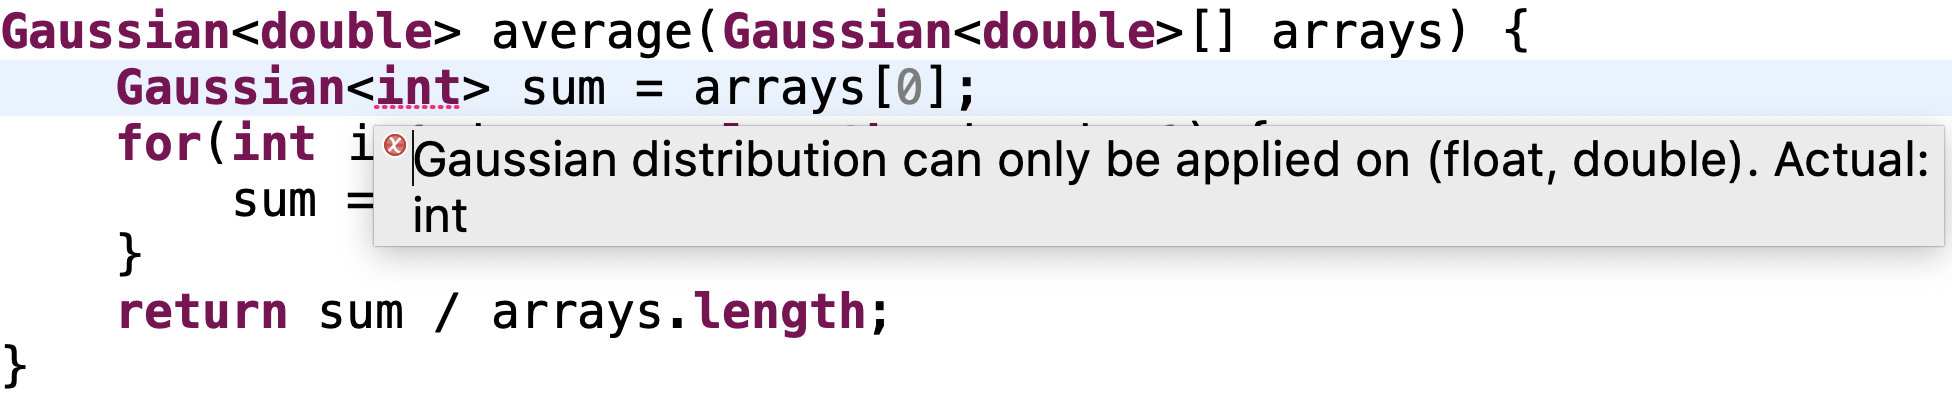
\includegraphics[width=\linewidth]{img/chapt-intro/approach/aintea-overview}
	\caption{Overview of the language proposed, \langName{}}
	\label{fig:intro:contrib:aintea}
\end{figure}

This contribution addresses the challenge of the manipulation of uncertain data (cf. Sub-Challenge \#1). 
We propose \langName{}, a language able to represent uncertain data as built-in language types along with their supported operations.
An overview of the language is depicted in~\Cref{fig:intro:contrib:aintea}.
 It contains a sampling of distributions (Gaussian, Bernoulli, binomial, Dirac delta function, and Rayleigh) that covers the different data types (booleans, numbers, and references).
 We implement a prototype of the language, publicly available on GitHub\footnote{\url{https://github.com/lmouline/aintea/}}.
 We use a real-world case study based on \gls{sg}, built with our partner Creos S.A..
It shows first that our approach does not impact the conciseness of the language.
Second, it highlights the feasibility and the advantages of uncertainty-aware type checking systems on the language level.

This contribution is under submission at the JOT Journal\footnote{\url{http://www.jot.fm/}}:
\begin{itemize}
	\item \citetitle{insubmission:2019:comlan:datauncertainty}, \citeauthor{insubmission:2019:comlan:datauncertainty}
\end{itemize}

\paragraph{A temporal knowledge \gls{metamodel}}
\begin{figure}
	\centering
	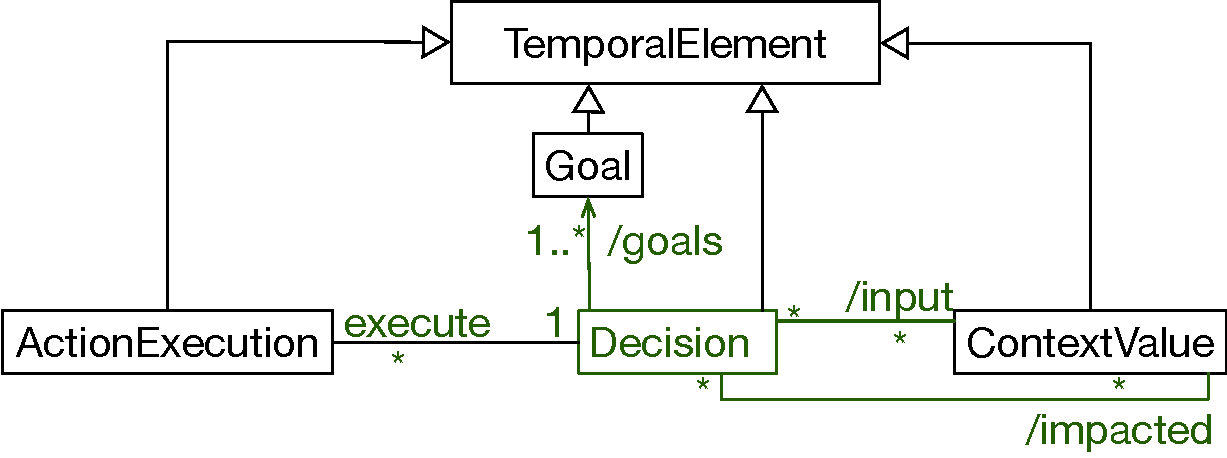
\includegraphics[width=0.6\linewidth]{img/chapt-intro/approach/tkm-overview}
	\caption{Overview of the temporal knowledge model}
	\label{fig:intro:contrib:tkm}
\end{figure}

This contribution addresses the challenge of reasoning over unfinished actions and of the understanding of \gls{adptSyst} \gls{behaviour} (cf. Sub-Challenge \#2 and \#3).
First, we formalise the common core concepts implied in adaptation processes, also referred to as \gls{knowledge}.
The formalisation is based on temporal graphs and a set of relations that trace decisions impact to circumstances.
Second, we propose a framework to structure and store the state and behaviour of a running \gls{adptSyst}, together with a high-level \gls{api} to efficiently perform diagnosis routines.
Our framework relies on a temporal model-based solution that efficiently abstracts decisions, their corresponding circumstances, and their effects.
We give an overview of the \gls{metamodel} in~\Cref{fig:intro:contrib:tkm}.
We demonstrate the applicability of our approach by applying it to a \gls{sg} based example.
We also show that our approach can be used to diagnose the behaviour of at most the last five days of a district in the Luxembourg \gls{sg} in $\sim$2.4 seconds.


Part of this contribution has been published at the IEEE International Conference on Autonomic Computing\footnote{\url{http://icac2018.informatik.uni-wuerzburg.de/}} (ICAC) and at the ACM/SIGAPP Symposium On Applied Computing\footnote{\url{http://www.sigapp.org/sac/sac2018/}} (SAC):
\begin{itemize}
	\item \citetitle{DBLP:conf/sac/MoulineB0FBMB18}, \citeauthor{DBLP:conf/sac/MoulineB0FBMB18}
	\item \citetitle{DBLP:conf/icac/MoulineBFBB18}, \citeauthor{DBLP:conf/icac/MoulineBFBB18}
\end{itemize}
\section{Structure of the document}

\begin{figure}
	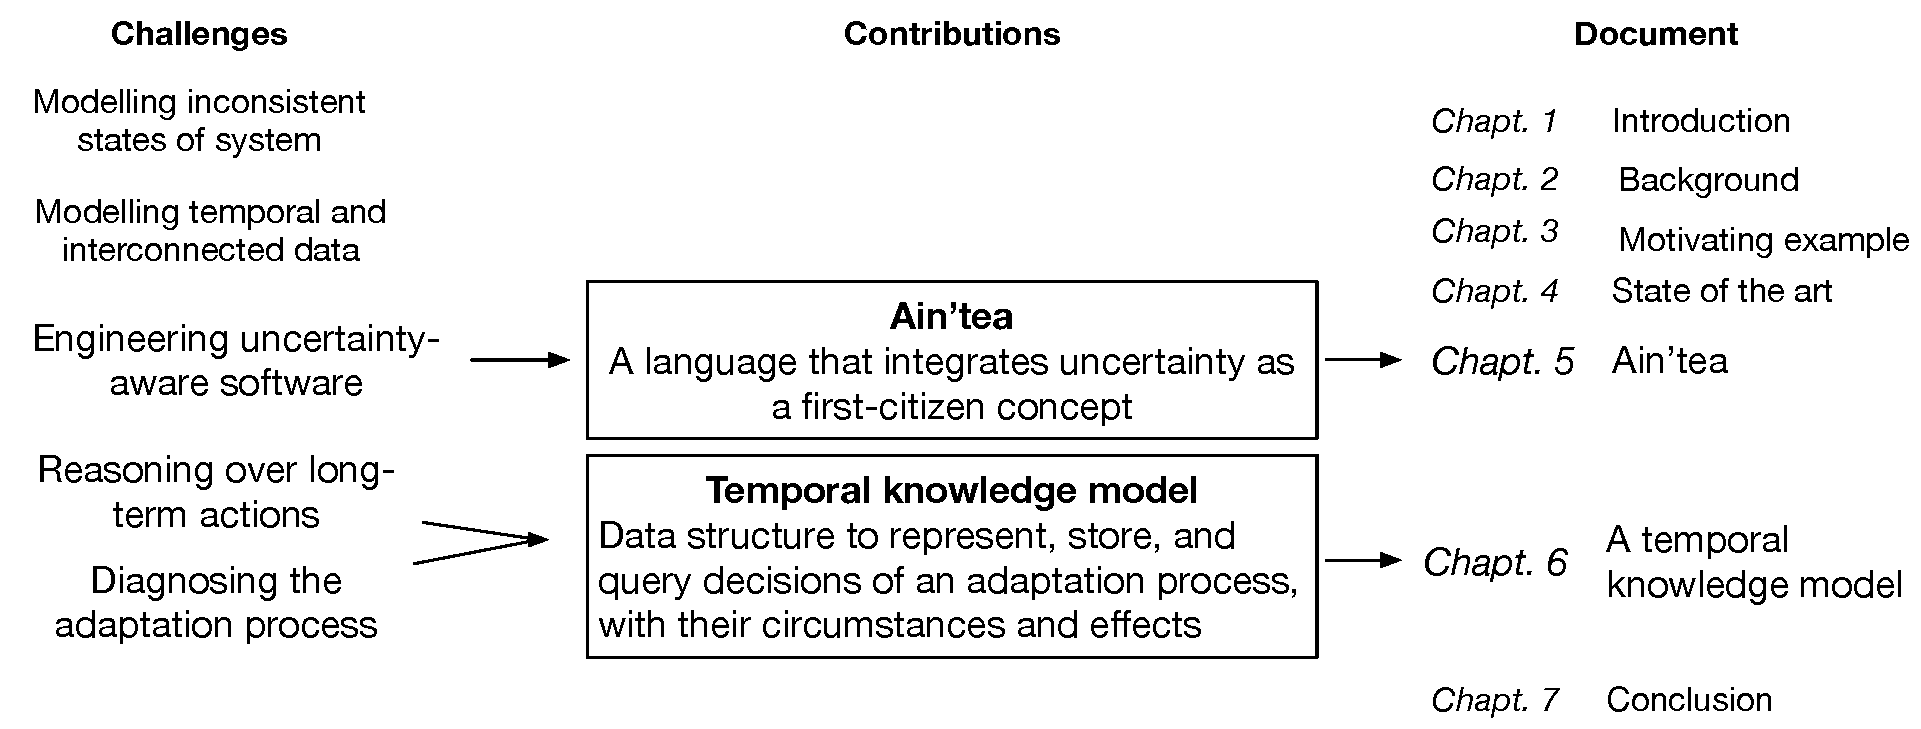
\includegraphics[width=\linewidth]{img/chapt-intro/struct/struct}
	\caption{Structure of the document}
	\label{fig:intro:structDoc}
\end{figure}

We split the remaining part of this document into six chapters, as shown in~\Cref{fig:intro:structDoc}.
First, \Cref{chapt:background} describes the necessary background of the thesis.
Then, \Cref{chapt:example} describes a motivating example, based on a \gls{sg} system.
We present concepts related to \gls{mde} and \glspl{adptSyst}.
Based on this background, we show the gap of the current state of the art in \Cref{chapt:sota}.
\Cref{chapt:aintea} and \Cref{chapt:tkm} described our two contributions.
The former details our language, \langName, that integrates uncertainty as a first-class citizen.
The latter explains our temporal \gls{metamodel} that can represent past and ongoing \glspl{action} with their circumstances and effects.
Finally, we conclude in \Cref{chapt:conclusion}, and we present a set of future works.
